
%  AppliNGS
%
%  Created by Valentin Loux on 2010-10-31.
%  Copyright (c) 2010 INRA. All rights reserved.

\documentclass{beamer}



\mode<presentation>
{
  \usetheme{Antibes}
  % or ...

  \setbeamercovered{transparent}
  % or whatever (possibly just delete it)
}

% Use utf-8 encoding for foreign characters
\usepackage[french]{babel} 
\usepackage[utf8]{inputenc}
\usepackage{times}
\usepackage[T1]{fontenc}
\usepackage{pgf}
\usepackage{pgfarrows,pgfnodes,pgfshade}

% Package for including code in the document
 \usepackage{listings}
 \usepackage{url}


%%%%%% Begin Document %%%%%%%%%%%%%

\title[Applications NGS] % (optional, use only with long paper titles)
{Applications biologiques des nouvelles techniques de séquençage}

%\subtitle
%{Une plateforme d'annotation de génomes bactériens}

\author[V. Loux] % (optional, use only with lots of authors)
{Valentin~Loux}

\institute[INRA-MIG] % (optional, but mostly needed)
{
  Unité Mathématique, Informatique et Génome\\
  INRA, Jouy en Josas
}

\date[2 Novembre 2010] % (optional, should be abbreviation of conference name)
{Formation NGS 2010}

\graphicspath{{Figures/}}
\pgfdeclareimage[height=0.5cm]{miglogo}{miglogo}
\logo{\pgfuseimage{miglogo}}


% Delete this, if you do not want the table of contents to pop up at
% the beginning of each subsection:
\AtBeginSection[]
{
  \begin{frame}<beamer>
    \frametitle{Outline}
    \tableofcontents[currentsection]
  \end{frame}
}


% If you wish to uncover everything in a step-wise fashion, uncomment
% the following command: 

%\beamerdefaultoverlayspecification{<+->}


\begin{document}
	
	
\begin{frame}
  \titlepage
\end{frame}

\begin{frame}
  \frametitle{Plan}
  \tableofcontents
  % You might wish to add the option [pausesections]
\end{frame}


\section{Introduction}

\begin{frame}
  \frametitle{}
	\begin{itemize}
		\item Les nouvelles techniques de sequençage offrent des possibilités en terme d'expérience et d'échelle quasi inconnue jusqu'à maintenant.
		\item	Cela renouvelle les approches en génomique, génomique comparée, diagnostique médical.\ldots
	\end{itemize}
\end{frame}


\section{Sequençage ADN} % (fold)
\label{sec:sequençage_resequençage_massif}



\subsection{Séquençage classique} % (fold)
\label{sub:séquençage_classique_}



\begin{frame}
	\frametitle{Séquençage génomes}
\begin{itemize}
	\item Changement d'échelle dans le séquençage
	\item 10, 20 ou 100 souches
	\item Généralement, pas de finition
	\item Problèmes récurrents de moyens informatiques et bioinformatiques
\end{itemize}
\end{frame}




\begin{frame}
	\frametitle{GEBA~: A Genomic Encyclopedia for Bacteria and Archaea}
\begin{itemize}
\item Projet du DOE - JGI
\item But : remplir les "trous" dans l'arbre des espèces bactériennes
\item Projet pilote avec une centaine de génomes
\item Annotation faite par des étudiants
\end{itemize}
\center{\small{\url{http://www.jgi.doe.gov/programs/GEBA/}}}
\end{frame}

% subsection s�quen�age_classique_ (end)

\subsection{Recherche de variants (SNPs et mutations)} % (fold)
\label{sub:decouverte_de_variants}
\begin{frame}
	\frametitle{1000 genomes project}
\begin{itemize}
\item A pour but de trouver tous les variants présents dans au moins 1\% de la population étudiée.
\item Projet pilote avec~: 
\begin{itemize}
	\item 160 individus en basse couverture (4x) 
	\item 6 individus en couverture haute (40 x)
\end{itemize}
\item Prévoient de séquencer 2500 individus.
\end{itemize}
\small{1000 Genomes Project Consortium et al. A map of human genome variation from population-scale sequencing. Nature (2010)}
\end{frame}


% subsection decouverte_de_variants (end)

\subsection{Métagénomique} % (fold)
\label{sub:métagénomique}

\begin{frame}
	\frametitle{Métagénomique}
\begin{itemize}
	\item Etudes de la diversité microbienne d'échantillons environnementaux ou de flore commensale~:
	\begin{itemize}
		\item Sols (éventuellement pollués)
		\item Boue d'épurations
		\item Océan
		\item Estomac, bouche, \ldots
	\end{itemize}
\end{itemize}
\end{frame}


\begin{frame}
	\frametitle{Métagenome intestinal}
\begin{itemize}
	\item "Autre" génome (100 fois plus de bacteries dans l'intestin que de cellules humaines)
	\item 124 individus européens
	\item 576,7 Gbase de séquences
	\item  3.3 millions de gènes microbiens non-redondants
\end{itemize}
\tiny{Qin et al. A human gut microbial gene catalogue established by metagenomic sequencing. Nature (2010)}
\end{frame}



\subsection{Capture, enrichissement et séquencage d'exons} % (fold)
\label{sub:subsection_name}



\begin{frame}
	\frametitle{Capture, enrichissement et sequencage d'"exomes"}
		\center{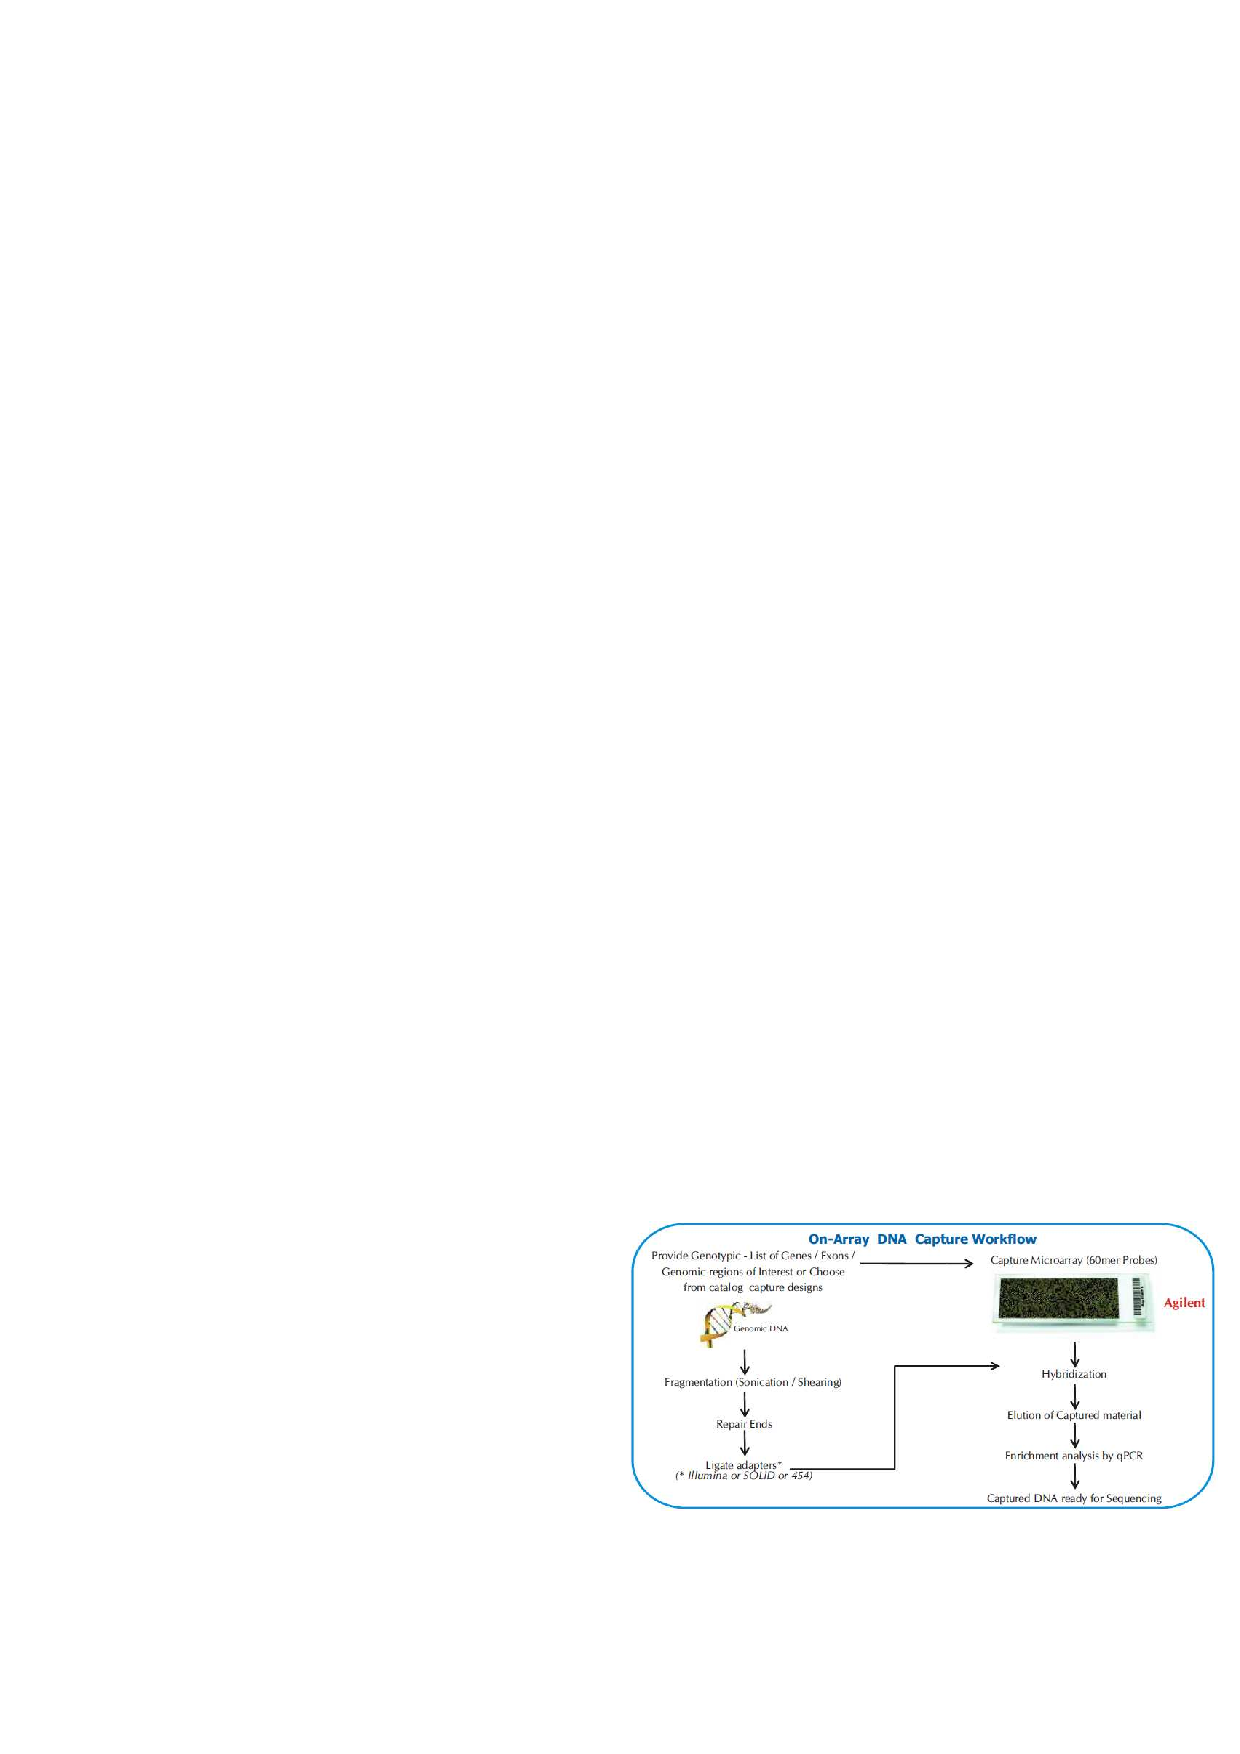
\includegraphics[width=\textwidth]{capture}}
		\tiny{Albert et al. Direct selection of human genomic loci by microarray hybridization. Nat Methods (2007)}
\end{frame}


% subsection subsection_name (end)
% subsection m�tag�nomique (end)

% section sequen�age_resequen�age_massif (end)



% subsection chip_seq_et_m�thylation (end)
\section{ChIP-Seq et Méthylation} % (fold)
\label{sec:capture_et_chip_seq}

\subsection{CHIP-Seq} % (fold)
%\label{sub:chip_seq_et_m�thylation}
\begin{frame}
	\frametitle{ChIP-SEQ}
		\center{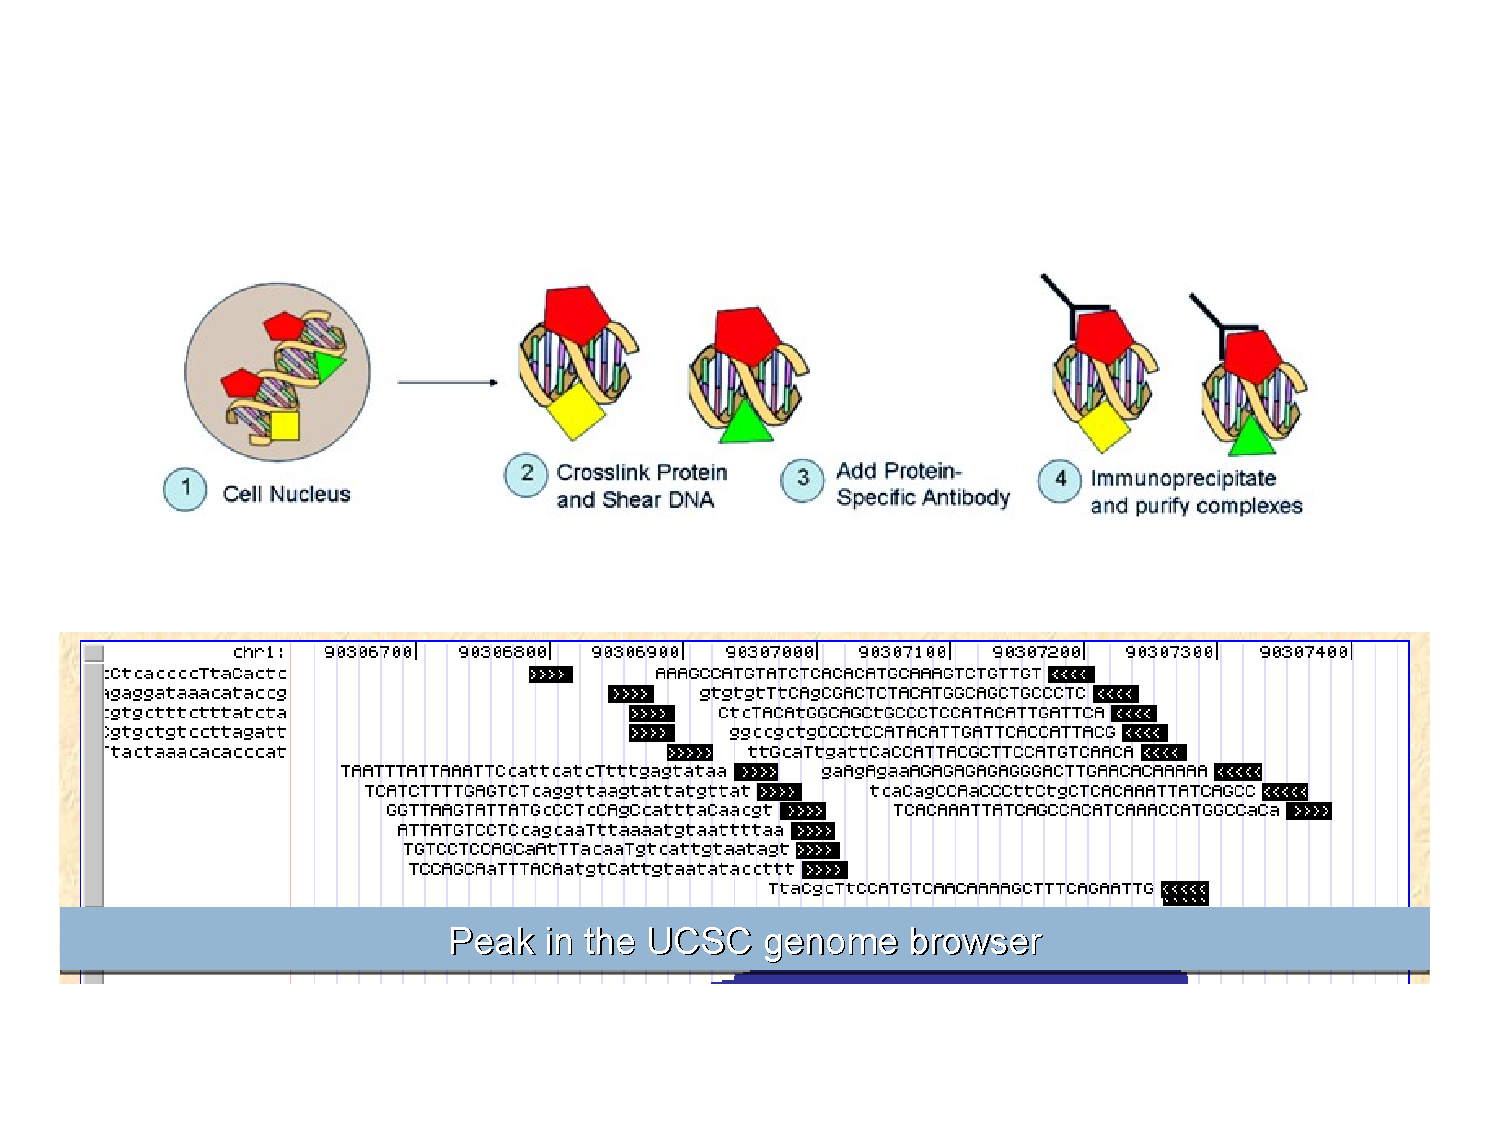
\includegraphics[width=\textwidth]{chipseq}}
		\tiny{© V. Boeva}\\
		\tiny{Jothi et al. Genome-wide identification of in vivo protein-DNA binding sites from ChIP-Seq data.\\ Nucleic Acids Res (2008)}
\end{frame}


\subsection{Méthylation} % (fold)
\label{sub:méthylation}


\begin{frame}
	\frametitle{Methylation}
		\center{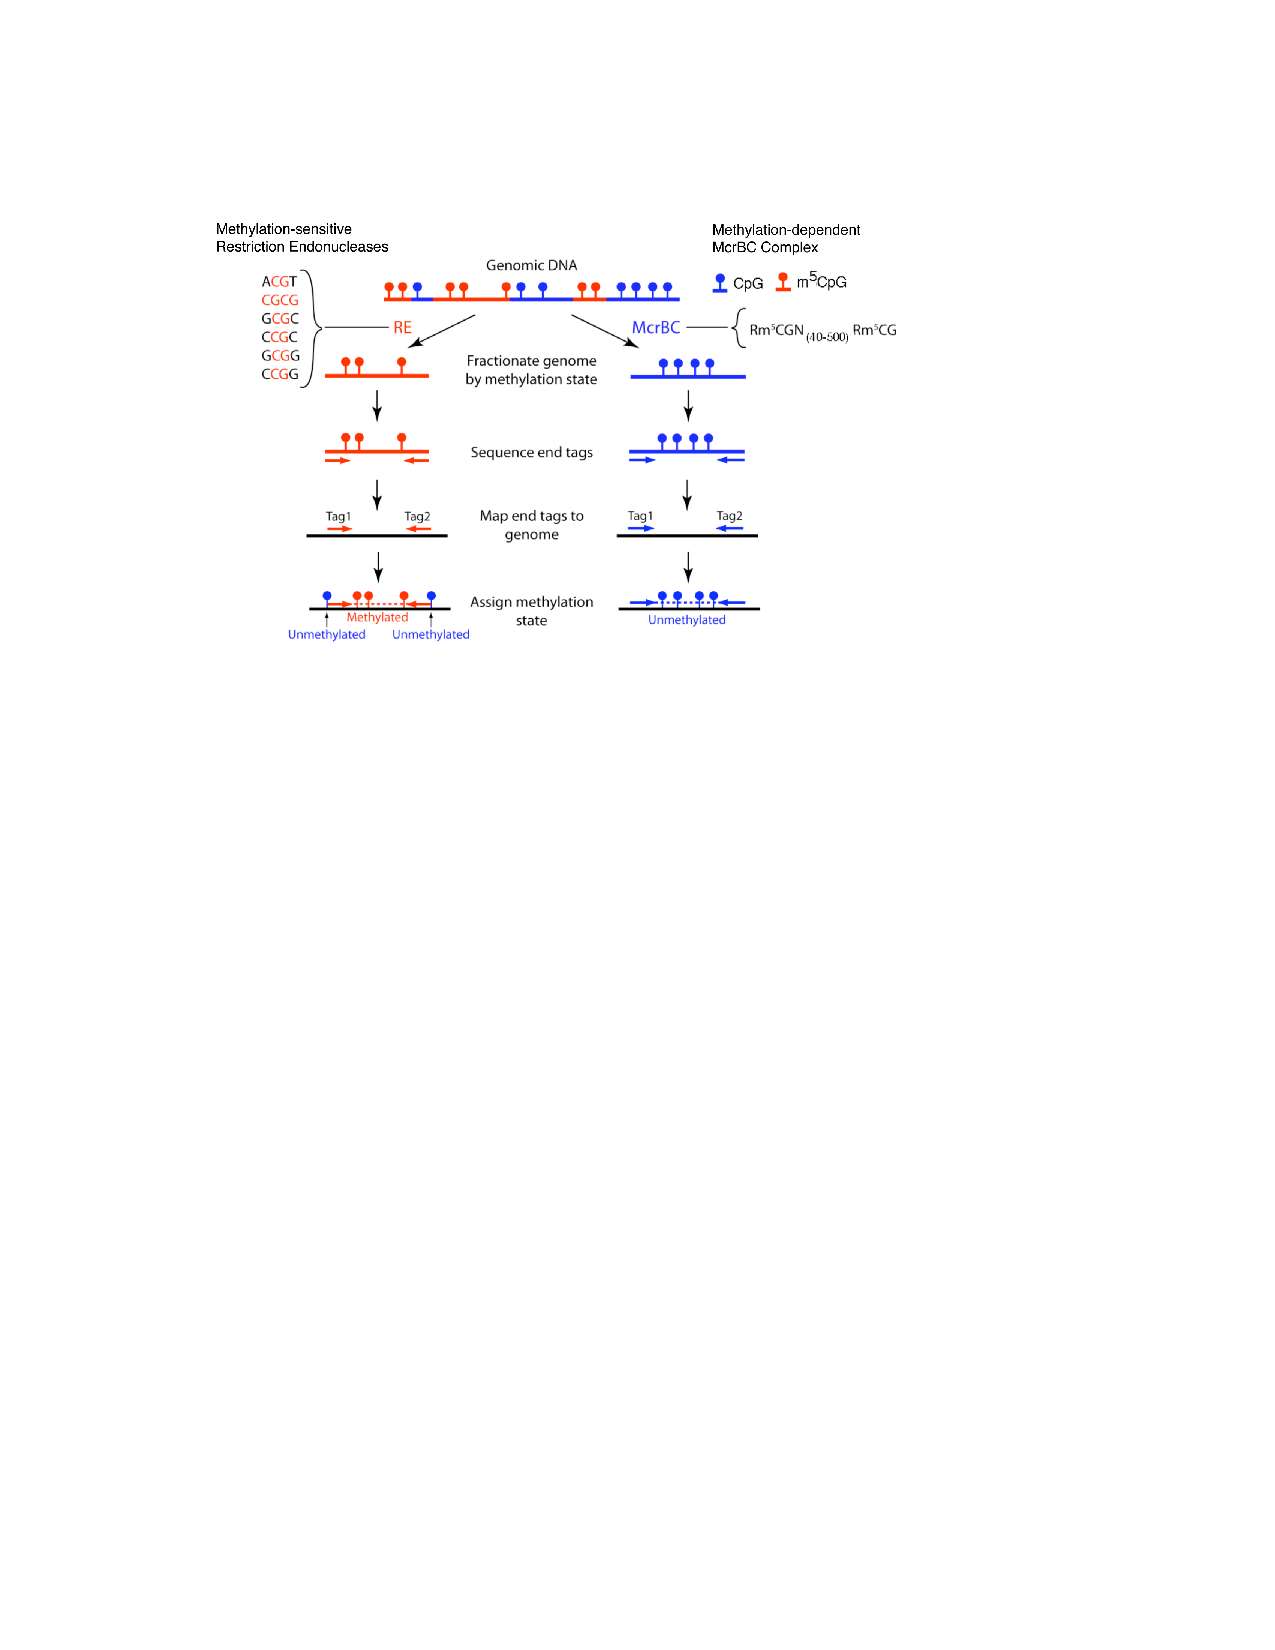
\includegraphics[width=\textwidth]{methylation}}
\tiny{Edwards et al. Chromatin and sequence features that define the fine and gross structure of genomic methylation patterns. Genome Res (2010)}
\end{frame}

% subsection m�thylation (end)


% Figure S1. Methyl-MAPS technique for whole-genome methylation analysis. Five methylation sensitive restriction enzymes (RE), that cut only unmethylated CpG sites, and McrBC, a methylation dependent endonuclease that cuts only methylated CpG sites, are used to fractionate the genome into methylated and unmethylated compartments, respectively. Millions of paired end-tags are sequenced for each compartment. Tag pairs are mapped to the genome and methylation state is assigned to end and interior CpG sites as appropriate. The tables show the number of CpG, McrBC, and RE sites found in the genome and in CpG islands in human (hg18) and mouse (mm9) genomes

% section capture_et_chip_seq (end)

\section{Transcriptomique} % (fold)
\label{sec:rnaseq_dge}
\subsection{Transcriptomique} % (fold)
\label{sub:transcriptomique}


\begin{frame}
	\frametitle{RNASeq}
		\center{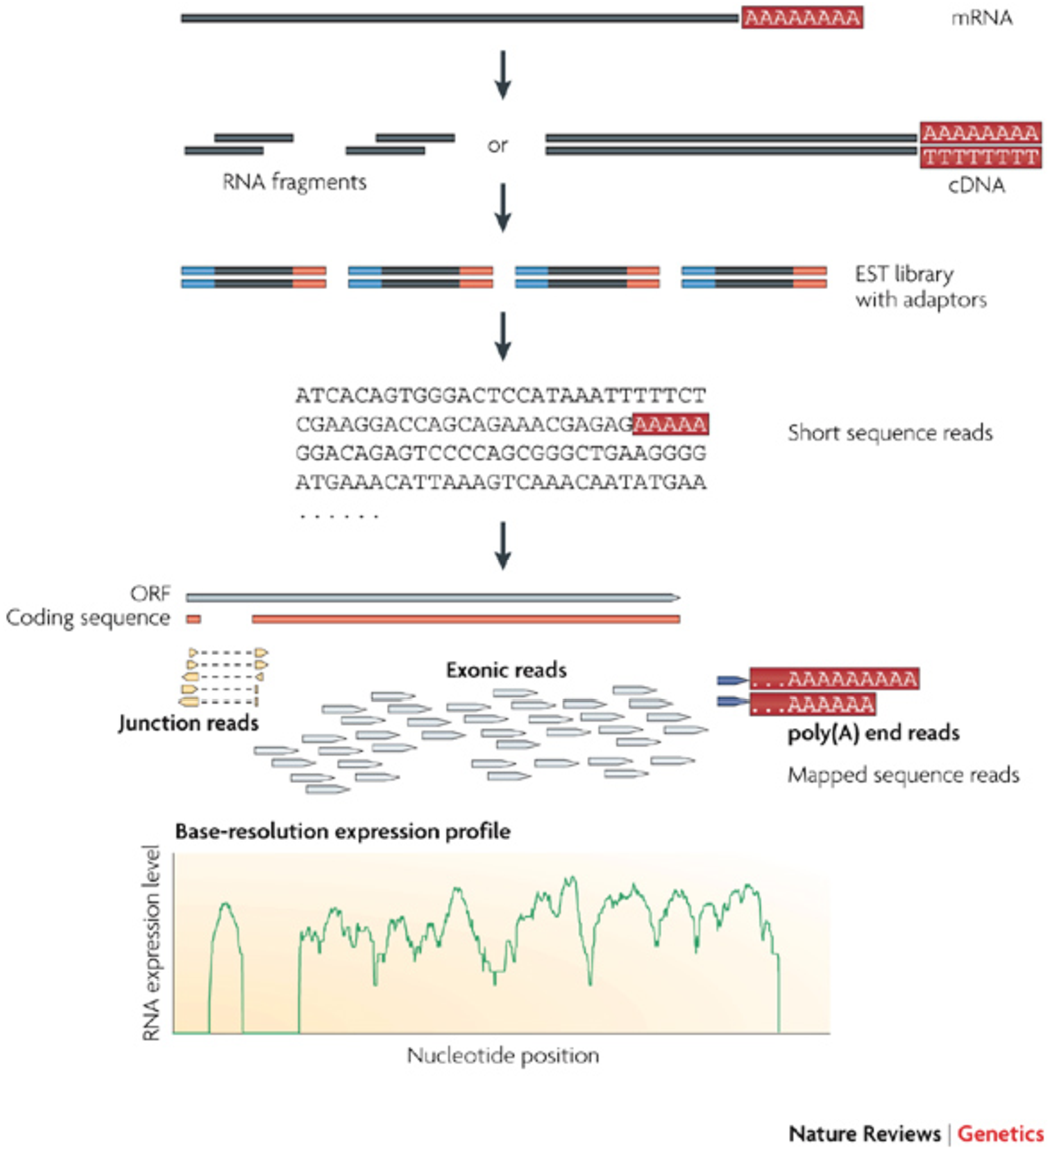
\includegraphics[height=7cm]{rnaseq}}
\end{frame}
% subsection transcriptomique (end)

\subsection{Digital Gene Expression} % (fold)
\label{sub:digital_gene_expression}

% subsection digital_gene_expression (end)
\begin{frame}
	\frametitle{DGE}
		\center{\includegraphics[height=7cm]{dge}}
\end{frame}


\begin{frame}
	\frametitle{DGE VS RNASeq}
		\center{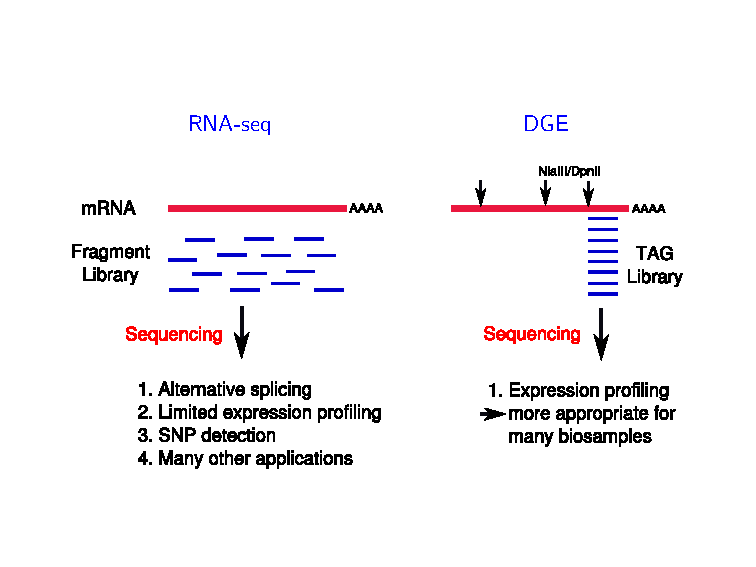
\includegraphics[width=\textwidth]{rnaseqVSDGE}}
\end{frame}
% section rnaseq_dge (end)


\section{Conclusion} % (fold)
\label{sec:conclusion}

% section conclusion (end)
\begin{frame}
	\frametitle{Conclusions}
	\begin{itemize}
		\item L'arrivé des nouvelles techniques de séquençage a permis le passage à des échelles insoupçonnées de techniques existantes (methylation, rnaSeq, 1000 génomes,\ldots)
		\item De nouveaux types d'expériences (CHIP-Seq, Exon Capture) 
		\item De nouvelles questions de recherches en bioinformatique et statistique
		\item De nouveaux défis informatiques\ldots
	\end{itemize}
\end{frame}

\begin{frame}
	\frametitle{Séquençage contre stockage}
		\center{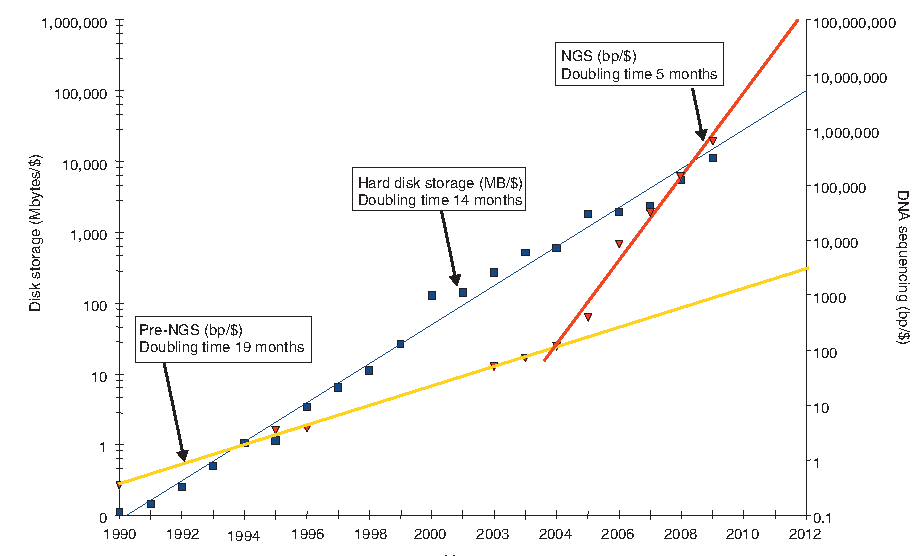
\includegraphics[width=\textwidth]{SteinNGS}}
\end{frame}

\begin{frame}
	\frametitle{Références}
\begin{itemize}
	\item Cock et al. The Sanger FASTQ file format for sequences with quality scores, and the Solexa/Illumina FASTQ variants. Nucleic Acids Res (2009)
	\item Qin et al. A human gut microbial gene catalogue established by metagenomic sequencing. Nature (2010)
	\item Stein. The case for cloud computing in genome informatics. Genome Biology 2010 11:207 (2010) vol. 11 (5) pp. 207
	\item 1000 Genomes Project Consortium et al. A map of human genome variation from population-scale sequencing. Nature (2010)
	
\item Jothi et al. Genome-wide identification of in vivo protein-DNA binding sites from ChIP-Seq data. Nucleic Acids Res (2008)



\end{itemize}
\end{frame}

\begin{frame}
	\frametitle{Références(2)}
\begin{itemize}
	\item Cokus et al. Shotgun bisulphite sequencing of the Arabidopsis genome reveals DNA methylation patterning. Nature (2008)
	\item Edwards et al. Chromatin and sequence features that define the fine and gross structure of genomic methylation patterns. Genome Res (2010)
	\item Albert et al. Direct selection of human genomic loci by microarray hybridization. Nat Methods (2007) vol. 4 (11) pp. 903-5
	\item Nature Review Genetics Series: Applications of next generation sequencing\\ \small{\url{http://www.nature.com/nrg/series/nextgeneration}}
\end{itemize}
\end{frame}

\end{document}
